\section{Context}\label{context}

Biogeographers are still debating about whether the biotic interactions
at the local scale impact large scale species distribution. If this is
indeed the case, then we should expect pairs of species to exhibit
non-random distribution at the large spatial scale. The observation of
independent species occurrences would therefore support the use of
classical species distribution models (hereafter SDMs,
\citet{Elith2006}) and confirm scenarios that have been proposed over
the last decade \citep{Thuiller2005, Thuiller2011, Albouy2012}, whereas
the observation of occurrence clearly related to interactions would give
credit to methods interpreting co-occurrence as a proxy for ecological
interactions \citep{Morales-Castilla2015} and encourage the use of joint
species distribution models \citep[hereafter
JSDM,][]{Ovaskainen2010, Pollock2014}. In order to test whether
interactions influence species distributions, the simplest avenue is to
investigate species co-distribution in light of their ecological
relationships. Such investigations started with Diamond's original study
stating that species interacting by competition should avoid each other
in space, leading to a `checkerboard' distribution \citep{Diamond1975}.
This idea was rapidly criticized for the lack of an adequate null
hypothesis \citep{Connor1979, Gilpin1982} and has led to a major
controversy that has lasted more than 30 \citep{Connor2013} and has
underlined the need for null models in ecology
\citep{Connor1983, Gotelli2000}. Furthermore, the absence of adequate
datasets has long prevent to test adequately this hypothesis.

Species ranges are very often inferred from the realized distribution,
which results from the joint impacts of abiotic and biotic environmental
factors along with dispersal limitations and historical contingencies
\citep{Pulliam2000, Holt2009, Godsoe2010a, Araujo2014}. Finding evidence
of the effect of species interactions on distribution may prove
technically difficult as it requires to discriminate the fundamental
niche from co-occurrence data (Box 1), which could explain the scarcity
of studies reporting such effect \citep[but see][]{Gotelli2010}.
Fortunately, recent developments in co-occurrence theory promises novel
avenues in which highly dimensional species distribution data could be
analyzed, accounting for the structure of the network of ecological
interactions \citep{Cazelles2016}. It has notably been proposed that the
higher the degree of a species, \emph{i.e} the number of species which
with it interacts, the weaker will be the detection of a signal of
co-occurrence. The geographical range of a species is indeed partially
correlated with all the ranges of species it is linked to, which should
blur the signal the interactions leave on pairwise co-occurrence,
however, a signal may persist in the co-occurrence of the focal species
with the joint distribution of the species it interacts with is
considered.\\
Also, two co-occurring species may be part of the same ecological
network but separated by several interactions, for such case, it has
been suggested that the longer the shortest-path, \emph{i.e} the number
of links between two species, the smaller the signal of co-occurrence.
Hence, based on co-occurrence data and information pertaining to
ecological network, the hypotheses recently formulated on the signal of
co-occurrence can be tested (Box 1).

Despite the fantastic number of studies investigating co-occurrence in
order to understand community assembly, the hypothesis that species
interactions should result in non-random associations in space has never
been tested formally. It is rather implicitly assumed in every
investigation. Our objective in this study is therefore to test this at
the scale of species range. We analyzed species association within five
different datasets ranging from plant-seed dispersers, host-parasitoids,
microbes, birds and forest trees. We quantify co-occurrence and
conditional co-occurrence accounting for abiotic constrains for species
that are known to interact and known to not interact directly. This is
an unique opportunity to test the hypotheses recently developed. We
report some signal of positive co-occurrence among the datasets,
suggesting a difference between pairs of interacting species and pairs
of not-interacting. We also point out that the degree of a species in a
network influences our ability to detect significant associations.
Moreover, we discover a clear relationship between the strength of
species associations and the cumulated occupancy of the entire set of
species with which a species interact. However, all the signal we
detected are weakened or even disappear once abiotic similarities among
site are integrated. We further discuss the integration of biotic
interactions in distribution models in the light of our results.

\section{Material and Methods}\label{material-and-methods}

\subsection{Datasets}\label{datasets}

We analyzed five datasets spawning a large diversity of organisms and
types of interactions (see \citet{tbl:id}), across an extensive gradient
of environmental conditions (see Fig S1 and SI Text). Our criteria for
selecting datasets were as follow: i) the occurrence data must have been
collected at the local scale, it could not be derived from range maps;
ii) data included observed absences; iii) occurrence was observed for
all species, not only a singe layer; interactions were known a priori;
v) since we are computing co-occurrences, which is typically a fairly
rare event, we needed an elevated number of sampling units. Direct
interactions were documented for four datasets and represented by
networks of ecological interactions: the Willow Leaf Network (WLN), the
Pitcher Plants Network (PPN), the Caribbean Hummingbirds Network (CHN),
the French Breeding Birds Survey (FBBS). We derived metawebs for each
network, \emph{i.e}, the matrix recording all interactions, and computed
three metrics among species from a regional pool: the connectance of
metawebs (proportion of realized interactions), the degree of species
(number of links for one species) and the shortest-path between all
pairs of species (the minimum number of link from one species to the
other, see SI Text). For the North American Trees (NAT) dataset, we
approximated competitive interactions by computing functional distance
between every pair of species (see table S1 and Fig S2). A similar proxy
for ecological interactions was also computed for the FBBS see table
S2). Only species that were present at least on 1\% of the total number
of observations were considered for the analysis (see SI Text).

\subsection{Quantifying co-occurrence}\label{quantifying-co-occurrence}

For each pair of species \(i\) and \(j\), we computed the number of
observed co-occurrence \(O_{i,j}\) and the expected number of
co-occurrence under independent distribution \(E_{i,j}\) and the
standard deviation associated \(SD_{i,j}\). We report the Z-score
\(O_{i,j}-E_{i,j}/SD_{i,j}\) \citep{Gilpin1982}, a standardized metric
of co-occurrence, with positive (negative) values indicating more (less)
co-occurrence relative to the random expectation. Expectations were
derived using three different methods. First, we assumed that all sites
were equivalent, meaning we ignored the potential influence of abiotic
conditions across the entire range. The observed co-occurrence is an
estimate computed from a limited number of observations
\citep{Gilpin1982, Veech2013} and therefore, we also considered an
hypergeometric distribution, which corrects for limited sample size (see
SI Text for further details). We used two different SDMs in order to
account for the abiotic environment and correct the random expectations,
namely, Generalized Linear Model (hereafter GLM) and Random Forest
(hereafter RF - see SI Text for more details and Fig S3 for the
assessment of models' performances). The correction using SDMs accounts
for the fact that species may co-occur simply because they have similar
abiotic requirements, irrespective of if they interact or not.

\section{Results}\label{results}

Without accounting the abiotic context, we observe a difference in the
strength of spatial associations between interacting and not-interacting
species (\ref{fig:synth} panels A to D, white boxplots) for two out of
four datasets for which direct interactions were known. In all cases,
spatial associations were positive, indicating that interacting species
are co-occurring more often that randomly expected, irrespective of the
type of interaction. For the WLN, distinguishing herbivore-willow
interactions from herbivore-parasitoids revealed that the strength of
co-occurrence was stronger for the former than the latter ones
(\ref{fig:shtpth} A-B). Interestingly, we noticed that the higher the
mean degree of species in the dataset, the more difficult the detection
of a signal of interactions in co-occurrence was (\ref{fig:shtpth} A-D).

We observed that the strength of spatial association was higher for
pairs of similar species (\ref{fig:synth} panels E and F) for the NAT
and FBBS datasets, for which we inferred a distance based on functional
traits. Functional similarity is often interpreted as a proxy for
competition strength \citep{Morales-Castilla2015}, which according to
Diamond's hypothesis, should provide a negative association. However,
the observed associations are rather positive for functionally similar
species. This suggest that local competition is poorly detectable at
large scale which is theoretically supported \citep{Araujo2014} and the
positive associations are likely the results of similar physiological
requirements that cannot be taken into account given the sets of abiotic
variables we used. This is further supported by the regressions of the
Z-score against the distance (see Fig. S6 A-D). We also note that
results for the FBBS dataset were identical irrespective the type of
traits examined (Fig. S4). When we account for suitability discrepancies
among sites, \emph{i.e.} when we perform SDMs, the co-occurrence signals
we previously observed are weakened or disappeared. Co-occurrence
distributions are shifted toward 0 and dramatically shrunk (Fig.
\ref{fig:synth} panels A to D, grey and dark grey boxplots). The
tendencies are stronger for the RF approach than for the GLM one. The
same trends are observed when we used functional distance rather that
interactions (Fig. \ref{fig:synth} panels E-F).

We investigated if the strength of associations between species
interacting indirectly decreases with the shortest path (Fig.
\ref{fig:shtpth}). We examined the co-occurrence distribution against
the shortest-path for pairs of: herbivores and willows in WLN (A),
herbivores and parasitoids in WLN (B), hummingbirds and hosts plants (C)
and all pairs in PPN (D). Without accounting for the climatic factors,
we observe a decrease of the standardized co-occurrence with an
increased shortest-path for three out of four occurrence datasets (Fig.
\ref{fig:shtpth} A-D, white boxplots). This was predicted by the theory,
but the observed decay is steeper than anticipated \citep{Cazelles2016}.
We observed a similar but weaker decay when all pairs of species were
taken into account (see Fig. S5). Moreover, when we calculated the mean
degree in of predators (pollinators), we also found the signal of
co-occurrence stronger for specialists (Fig. \ref{fig:shtpth} A) than
for generalists (Fig. \ref{fig:shtpth} C), suggesting that the abundance
of interactions may prevent us from detecting them in static occurrence
data. Again, the tendencies observed are strongly weakened when
occurrence probability are derived from SDMs (Fig. \ref{fig:shtpth} A-D
grey and darker grey boxplots).

Finally, for all predators and pollinators in WLN, CHN and PPN, we
average the standardized co-occurrence over the set of their respective
preys (host plants) and plotted the obtained values against the total
number of site covered by the same set of preys (hosts) they refer to
(\ref{fig:degocc}). When abiotic context is not included, we observe a
clear negative relationship between the two quantities for three out of
four datasets. The associated linear regressions explain up to 69\% of
the variance (\ref{fig:degocc} panels A, D, G and J). However, the
linear regression poorly performed for the PPN, in which the connectance
is the highest. Additionally, we show that the linear regressions
outperformed the ones using the degree of the species (Fig S7 panels A,
D, G and J) that was envisioned by the theory \citep{Cazelles2016}.
Moreover, the relation is asymmetric: the decay is less convincing when
the the mean Z-scores of the preys are plotted against the cumulated
range of their predators (fig S8 panels A, D, G and J). These results
suggest that for a predator (pollinator) feeding upon a set of preys
(hosts), the detection of interactions is possible if the part of the
geographic range studied covered by the preys is low, when the part
increases our ability to detect the signal fades away. Once again, the
results are dramatically different once abiotic constrains were taken
into account: the clear relationship obtained is either weakened or even
reversed (\ref{fig:degocc} B,C,E,F,H,I,K,L). Even the strongest
associations seem to be captured by the SDMs, meaning they are captured
by the link with this environment but this questions how the inference
is made when the presence of one species is best explained by the
presence of its prey. Indeed, we show the presence of the whole set of
prey as predictor to assign the presence of specialist predator
outperform GLMs but not RFs (see Fig. S9).

\subsection{Discussion}\label{discussion}

The historical debate on co-occurrence triggered by Diamond's original
work was based on the idea that competitors must repulsed each other
\citep{Diamond1975}. Interestingly, we were not able to detect any
negative signal for species we assumed to compete. This support the idea
that local repulsion that must occur do not leave any mark on
co-occurrence data over a broad geographical gradient
\citep{Araujo2014}. However, we demonstrate that other signals, not
mentioned in the controversy, can actually be revealed. Mutualism and
predation were indeed detected as positive signals in the standardized
co-occurrence. Therefore, the interdependency between a predator
(pollinator) and its preys (host plant) makes them co-occurring more
than randomly expected and this effect is appreciable at large scale
\citep{Araujo2014}. Moreover, we find that the signal of co-occurrence
is blurred by the number of interactions a species experience, in
agreement with recent co-occurrence theory \citep{Cazelles2016}. As a
consequence, the distribution of a given species is more strongly
related to the distribution of the entire set of species it interacts
with, than each species taken individually. This indicates that the role
of ecological interactions may not only be a matter of spatial scale
\citep{McGill2010}, but also a matter of picking the most consistent
biological unit to investigate distribution over large spatial scales.

The signal of co-occurrence were dramatically reduced once we accounted
for the abiotic context. This could lead us to conclude that
co-occurrences are likely driven by the abiotic difference among site.
Climatic data doubtlessly explains a large part of the co-occurrence
observed, however our findings suggest a potential methodological issue.
Current SDMs always use abiotic constraints as the main drivers of
geographic distributions. In doing so, they capture, at least partially,
the impact of biotic interactions on distribution (as it infers the
distribution from the realized distribution). A predator is therefore
linked to its preys through the abiotic similarities of the sites where
they are found. However, the strength of an association may not be
perfectly captured by SDMs, this would explain why the relationship
vanishes in \ref{fig:degocc} when we used SDMs approach to derive
co-occurrence probabilities while the co-occurrence signal remains
positive. Understanding which part of the interactions is captured by
the SDMs remains of central important to build better distribution
models.

SDMs are based on the assumption that species are distributed
independently from each other and that scenarios of tomorrow's
biodiversity can be anticipated using abiotic variables only
\citep{Jeschke2008}. Some recent developments in statistics relaxed this
hypothesis by representing the distribution of assemblages, based on
correlations between species \citep{Pollock2014, Warton2015b}. The
development of these powerful statistical tools is essential, however it
can only provide a partial solution to some limitations of SDMs.\\
A substantial part of the solution lies in the understanding of the role
of ecological and evolutionary mechanisms shaping distributions
\citep{Thuiller2013}. Here, we underline the need for not hypothesizing
\emph{a priori} the independence among species. Rather, the assumption
must be proved to apply, otherwise a relevant assemblage must be
modeled. We suggest that for generalist species, the assumption of
independence is reasonable while for specialists the relative position
with the other species within the network should help deciding which set
of species are to be modeled. We therefore suggest that ecological
interactions should be integrated as prior information in SDMs to
strengthen our predictions. For instance, the range of a predator is
bounded by the range of the set of its preys
\citep{Holt2009, Shenbrot2007}, this reality should be integrated into
account when we predict the distribution of food webs, and predators'
ranges must be computed consistently with the predicted ranges of their
prey.

Our results lead us to conclude that co-occurrence tends to the
independence with increasing diversity of interactions. Only the
specialized species are strongly associated with their partners, as
generalists experience a much more diffuse constraint from interacting
species. Similarly, it it has been recently highlighted that net species
interaction strength better pairs of species is better predicted when
the species richness increases \citep{Berlow2009}. Further, press
perturbations applied to specialist species do have much stronger
indirect impacts on the other species than perturbations applied to
generalists \citep{Montoya2009}. All of these results are congruent with
MacArthur's vision, who more than 40 years ago, noticed the following
paradox \emph{``How can a more complex community be easier to
understand? A possible answer might be that the complex community have
strong interactions among species so that the lives of the separate
species are less independent than in a simple community. Where there is
greater interdependence, patterns may be more conspicuous.''}
\citep[p.199]{macarthur1972geographical}. In the present study, the more
the interactions among species the easier the forecasting of species
distribution. However, under the ongoing mass extinction, a myriad of
links vanishes while new ones emerge with the changes in the composition
of local communities. Therefore, even if under current conditions the
assumption of independence may be valid, under dramatic modifications of
ecosystem as currently observed, it may often prove false. As a step
forward, new biodiversity scenarios must not solely map the future
ranges of individual species but the entire community including the
consequences of potential extinction on community structure.

\newpage

\subsection{Box 1}\label{box-1}

The fundamental niche is here defined as the occurrence probability
under the assumptions that (1) biotic factors are not limiting the
occupancy and (2) the occupancy is estimated in the absence of
immigration \citep{Godsoe2010a}. In this case, only abiotic factors
(such as water availability, temperature variability or edaphic
variables) limit survival and/or reproduction success, and then the
occurrence probability. For a four species network made of three trophic
levels: two primary producers, a predator feeding upon them and a top
predator, we first consider the fundamental niches \(f_i\)
(\ref{fig:box1} A). For the top predator, we derive the fundamental
niche under the assumption of the presence of its prey:

\[f_4(w)=P(X_4=1|X_3=1, G=w)\]

where \(G\) denotes the environmental gradient and \(X_i\) represents
the random variable of the presence of species \(i\). For the lower
predator, we consider its preys substitutable and we assume the presence
of at least one prey to allow the predator to be present:

\[f_3(w)=P(X_3=1|X_2+X_1>0, G=w)\]

Similarly, \(f_1\) and \(f_2\) are obtained assuming that 3 is absent:

\[f_2(w)=P(X_2=1|X_3=0, G=w)\]

and:

\[f_1(w)=P(X_1=1|X_3=0, G=w)\]

Once projected on a map, the fundamental niche unravels the potential
distribution of a species \citep{Kearney2004}. The expected distribution
can be compared to real observations and could reveal whether dispersal
limits and ecological interactions are prevalent in the occupancy
dynamics of studied species. The realized niche (\ref{fig:box1} B)
includes these factors.\\
In our simplified example, fundamental and realized niches of preys are
identical. The realized niche of the top predator is constrained by the
one of predator 3, \(r_3\), which it-self is constrained by the joint
realized niches of its preys:

\[r_3(w)=P(X_3=1|X_2+X_1>0, G=w)P(X_2+X_1>0, G=w)\]
\[r_3(w)=f_3(w)\left(1-(1-r_1(w))(1-r_2(w))\right)\]

Then, assuming that species 4 do not alter \(r_3\), we have:

\[r_4(w)=f_4(w)r_3(w)\]
\[r_4(w)=f_4(w)f_3(w)\left(1-(1-r_1(w))(1-r_2(w))\right)\]

The above expressions may often be more complicated due to immigration
fluxes as well as the size and the structure of the interaction network.
For instance, we do not consider the apparent competition between
species 1 and 2, although it must affect their co-distribution.
Integrating the impact of many interactions may be possible using
occurrence probabilities of species assemblages rather than single
species \citep{Cazelles2016}. Here, the realized niches of predators 3
and 4 depends on the fundamental niches of preys 1 and 2.

The link between the fundamental niche and the distribution goes through
different ecological processes such as immigration and ecological
interaction \citep{Pulliam2000, Godsoe2010a}. The distribution we infer
is based on realized niche that includes the effect of abiotic variables
and biotic interactions. If we now examine the co-occurrence signals,
\emph{i.e.} the difference between the expected co-occurrence and the
observed co-occurrence \citep{Cazelles2016}, in empirical data, in order
to ascribe a particular signal to an ecological interaction, five
difficulties emerge:

\begin{enumerate}
\def\labelenumi{\arabic{enumi}.}
\tightlist
\item
  the signal of co-occurrence is not constant along the environmental
  gradient (\ref{fig:box1} C-a),
\item
  for species experiencing several interactions, the association with a
  particular species may be detectable only for a portion of the
  environmental gradient (\ref{fig:box1} C-b)
\item
  for species experiencing several interactions, the signal of
  co-occurrence with the set of species it interacts with might be more
  informative (\ref{fig:box1} C-c),
\item
  for species experiencing several interactions, the increase of
  interaction weakens the signal (this explain the drop for medium
  environmental values in \ref{fig:box1} C-c),
\item
  when the shortest-path between two species increase, the signal
  decreases (the red lines in \ref{fig:box1} C-c) is below the grey
  one).
\end{enumerate}

Using datasets including occurrence data for a large number of species
together with information pertaining to the ecological relationships, we
propose to test these theoretical expectations.

\newpage

\subsection{Tables}\label{tables}

\begin{longtable}[]{@{}lrrrrrrr@{}}
\caption{Data sets analyzed in this article.
\label{tbl:data}}\tabularnewline
\toprule
\begin{minipage}[b]{0.15\columnwidth}\raggedright\strut
Type\strut
\end{minipage} & \begin{minipage}[b]{0.07\columnwidth}\raggedleft\strut
No. of sites\strut
\end{minipage} & \begin{minipage}[b]{0.07\columnwidth}\raggedleft\strut
No. of species\strut
\end{minipage} & \begin{minipage}[b]{0.11\columnwidth}\raggedleft\strut
Interaction type\strut
\end{minipage} & \begin{minipage}[b]{0.05\columnwidth}\raggedleft\strut
Observed\strut
\end{minipage} & \begin{minipage}[b]{0.04\columnwidth}\raggedleft\strut
Traits\strut
\end{minipage} & \begin{minipage}[b]{0.06\columnwidth}\raggedleft\strut
Connectance\strut
\end{minipage} & \begin{minipage}[b]{0.22\columnwidth}\raggedleft\strut
References\strut
\end{minipage}\tabularnewline
\midrule
\endfirsthead
\toprule
\begin{minipage}[b]{0.15\columnwidth}\raggedright\strut
Type\strut
\end{minipage} & \begin{minipage}[b]{0.07\columnwidth}\raggedleft\strut
No. of sites\strut
\end{minipage} & \begin{minipage}[b]{0.07\columnwidth}\raggedleft\strut
No. of species\strut
\end{minipage} & \begin{minipage}[b]{0.11\columnwidth}\raggedleft\strut
Interaction type\strut
\end{minipage} & \begin{minipage}[b]{0.05\columnwidth}\raggedleft\strut
Observed\strut
\end{minipage} & \begin{minipage}[b]{0.04\columnwidth}\raggedleft\strut
Traits\strut
\end{minipage} & \begin{minipage}[b]{0.06\columnwidth}\raggedleft\strut
Connectance\strut
\end{minipage} & \begin{minipage}[b]{0.22\columnwidth}\raggedleft\strut
References\strut
\end{minipage}\tabularnewline
\midrule
\endhead
\begin{minipage}[t]{0.15\columnwidth}\raggedright\strut
Willow Leaf Network\strut
\end{minipage} & \begin{minipage}[t]{0.07\columnwidth}\raggedleft\strut
374\strut
\end{minipage} & \begin{minipage}[t]{0.07\columnwidth}\raggedleft\strut
156\strut
\end{minipage} & \begin{minipage}[t]{0.11\columnwidth}\raggedleft\strut
Trophic / Parasitism\strut
\end{minipage} & \begin{minipage}[t]{0.05\columnwidth}\raggedleft\strut
yes\strut
\end{minipage} & \begin{minipage}[t]{0.04\columnwidth}\raggedleft\strut
no\strut
\end{minipage} & \begin{minipage}[t]{0.06\columnwidth}\raggedleft\strut
0.042\strut
\end{minipage} & \begin{minipage}[t]{0.22\columnwidth}\raggedleft\strut
unpublished\strut
\end{minipage}\tabularnewline
\begin{minipage}[t]{0.15\columnwidth}\raggedright\strut
Pitcher Plants Network\strut
\end{minipage} & \begin{minipage}[t]{0.07\columnwidth}\raggedleft\strut
39x20\strut
\end{minipage} & \begin{minipage}[t]{0.07\columnwidth}\raggedleft\strut
53\strut
\end{minipage} & \begin{minipage}[t]{0.11\columnwidth}\raggedleft\strut
Trophic\strut
\end{minipage} & \begin{minipage}[t]{0.05\columnwidth}\raggedleft\strut
yes\strut
\end{minipage} & \begin{minipage}[t]{0.04\columnwidth}\raggedleft\strut
no\strut
\end{minipage} & \begin{minipage}[t]{0.06\columnwidth}\raggedleft\strut
0.44\strut
\end{minipage} & \begin{minipage}[t]{0.22\columnwidth}\raggedleft\strut
\citet{Baiser_2011}\strut
\end{minipage}\tabularnewline
\begin{minipage}[t]{0.15\columnwidth}\raggedright\strut
Caribbean Hummingbirds Network\strut
\end{minipage} & \begin{minipage}[t]{0.07\columnwidth}\raggedleft\strut
32\strut
\end{minipage} & \begin{minipage}[t]{0.07\columnwidth}\raggedleft\strut
62\strut
\end{minipage} & \begin{minipage}[t]{0.11\columnwidth}\raggedleft\strut
Mutualist\strut
\end{minipage} & \begin{minipage}[t]{0.05\columnwidth}\raggedleft\strut
yes\strut
\end{minipage} & \begin{minipage}[t]{0.04\columnwidth}\raggedleft\strut
no\strut
\end{minipage} & \begin{minipage}[t]{0.06\columnwidth}\raggedleft\strut
0.011\strut
\end{minipage} & \begin{minipage}[t]{0.22\columnwidth}\raggedleft\strut
\citet{MartinGonzalez2015}, \citet{Sonne2016}, \citet{Lack1973}\strut
\end{minipage}\tabularnewline
\begin{minipage}[t]{0.15\columnwidth}\raggedright\strut
North American Trees\strut
\end{minipage} & \begin{minipage}[t]{0.07\columnwidth}\raggedleft\strut
128891\strut
\end{minipage} & \begin{minipage}[t]{0.07\columnwidth}\raggedleft\strut
31\strut
\end{minipage} & \begin{minipage}[t]{0.11\columnwidth}\raggedleft\strut
Competition\strut
\end{minipage} & \begin{minipage}[t]{0.05\columnwidth}\raggedleft\strut
yes\strut
\end{minipage} & \begin{minipage}[t]{0.04\columnwidth}\raggedleft\strut
no\strut
\end{minipage} & \begin{minipage}[t]{0.06\columnwidth}\raggedleft\strut
-\strut
\end{minipage} & \begin{minipage}[t]{0.22\columnwidth}\raggedleft\strut
unpublished\strut
\end{minipage}\tabularnewline
\begin{minipage}[t]{0.15\columnwidth}\raggedright\strut
French Breeding Birds Survey\strut
\end{minipage} & \begin{minipage}[t]{0.07\columnwidth}\raggedleft\strut
2354\strut
\end{minipage} & \begin{minipage}[t]{0.07\columnwidth}\raggedleft\strut
179\strut
\end{minipage} & \begin{minipage}[t]{0.11\columnwidth}\raggedleft\strut
Trophic\strut
\end{minipage} & \begin{minipage}[t]{0.05\columnwidth}\raggedleft\strut
yes\strut
\end{minipage} & \begin{minipage}[t]{0.04\columnwidth}\raggedleft\strut
no\strut
\end{minipage} & \begin{minipage}[t]{0.06\columnwidth}\raggedleft\strut
0.018\strut
\end{minipage} & \begin{minipage}[t]{0.22\columnwidth}\raggedleft\strut
\citet{Gauzere2015}\strut
\end{minipage}\tabularnewline
\bottomrule
\end{longtable}

\newpage

\section{Figures}\label{figures}

\begin{figure}[htbp]
\centering
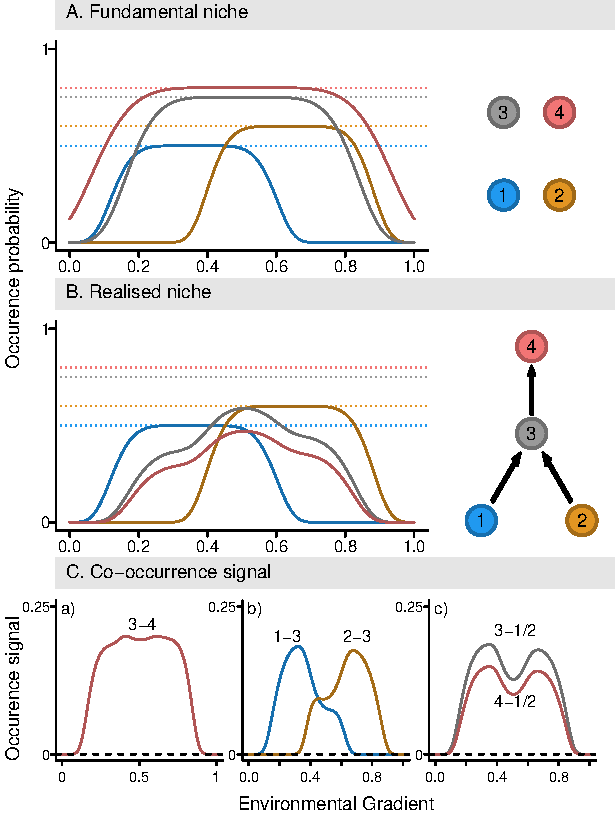
\includegraphics{../fig/figConcept.pdf}
\caption{\textbf{Probabilistic description of fundamental and realized
niches} For a four species network, all the occurrence probabilities are
derived along an environmental gradient assuming that (A) interactions
are not limiting the distribution and (B) that predators 3 and 4 needs
at least of one of its preys, \emph{i.e.} species 1 or 2. Horizontal
dotted lines in (A) and (B) stand for the occurrence probabilities
reached at an environmental optimum. The co-occurrence signal is
calculated for the following pairs : a) predators 3 and 4; b) predator 3
and prey 1, predator 3 and prey 1; c) predator 3 and prey 1 or 2,
predator 4 and prey 1 or 2. If no difference are found, 0 is
expected.\label{fig:box1}}
\end{figure}

\newpage

\begin{figure}[htbp]
\centering
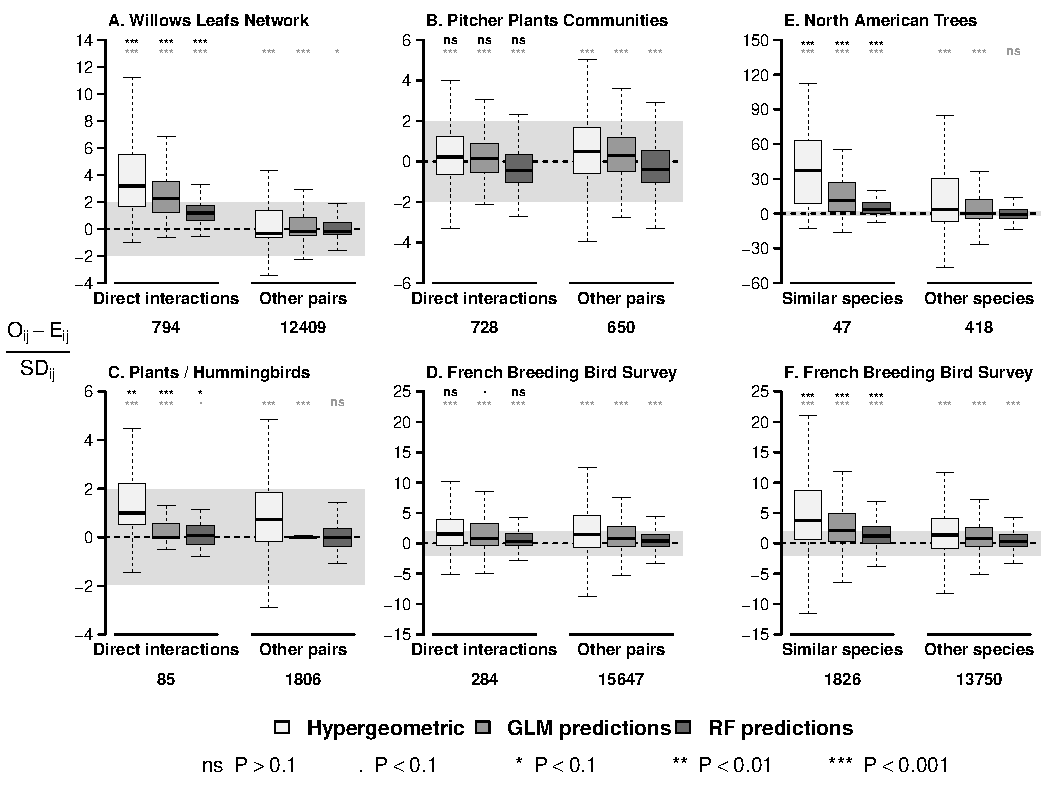
\includegraphics{../fig/figIntVsNoint.pdf}
\caption{\textbf{Co-occurrence of interacting versus not-interacting
pairs of species} Figures under each groups of boxplots indicate the
number of pairs to which the Z-score distributions refer. The light grey
rectangle corresponds to the 95\% confidence interval for the standard
normal distribution which gives insight into the proportion of pairs of
species significantly different from 0. The comparison made in panels A
to D is based on direct interactions observed. For panels E and F,
similar species are defined as the species for which the trait-based
distance is less than or equal to the lower decile of this distance
distribution. Note that outliers are not displayed. P values were
computed using the Wilcoxon rank sum test, to compare interacting versus
not-interacting Z-score distribution calculated for the three different
methods (black symbols) and to show whether the distribution is
symmetric about 0 (light grey symbols).\label{fig:synth}}
\end{figure}

\newpage

\begin{figure}[htbp]
\centering
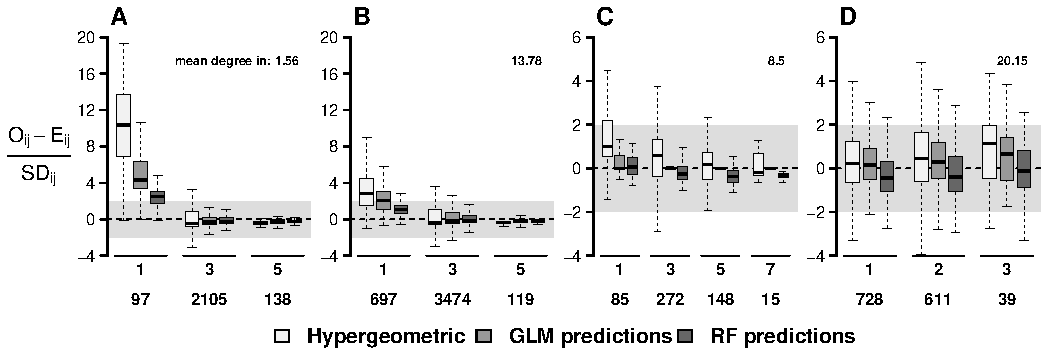
\includegraphics{../fig/figOrder.pdf}
\caption{\textbf{Co-occurrence signal decays when the shortest path
between a pair of species decay } The Z-score distribution are plotted
against the shortest path for A willows-herbivores interactions, B
herbivores-parasitoids interactions, C birds-plants interactions and D
the pitcher plants network. First figures under each grouped boxplots
indicate the shortest path associated while the figures below provide
the number of pair to which the distribution refers. Note that we used
the same y-axis for panels A and B as they regard two different kind of
interaction of the same dataset.\label{fig:shtpth}}
\end{figure}

\newpage

\begin{figure}[htbp]
\centering
\includegraphics{../fig/figdegocc.pdf}
\caption{\textbf{Co-occurrence significance decreases as the cumulated
occupancy increases} For a given species, Z-scores are averaged over the
all set species it interacts with and plotted against the joint
distribution of the same set of species. We do so for the herbivores in
the willows leafs network (panels A to C), the parasitoids in the willow
leafs network (panels D to F), the hummingbirds in the Caribbean
hummingbirds datasets (panels G to I) and all species in the pitcher
plants network that consume other species (panels J to L). The x-axis is
expressed as a log proportion of the total number of sites. Black
symbols are mean Z-scores significantly different from 0 (see SI Text).
In each panel, the dotted line represents the linear regression
\(y~ax+b\) for which the \(R^2\) is provided. The size of circles
reflects the degree of species for which the Z-score was calculated, the
relation size-degree for each row is given in the middle panel. For the
hummingbirds dataset (panels G to I), the triangle represent the values
obtained for the former distribution of a species already analyzed (see
SI text).\label{fig:degocc}}
\end{figure}

\newpage
